\documentclass[12pt]{article} 

\usepackage{natbib,hyperref,graphicx}
\usepackage[separate-uncertainty=true,multi-part-units=single]{siunitx}

\usepackage[margin=1.5cm, left=3cm ,twoside]{geometry}

\usepackage[para]{footmisc}


\DeclareSIUnit{\arcsec}{''}
\DeclareSIUnit{\mag}{\text{mag}}

\usepackage[utf8]{inputenc}
\usepackage{newunicodechar}

\DeclareRobustCommand{\okina}{%
  \raisebox{\dimexpr\fontcharht\font`A-\height}{%
    \scalebox{0.8}{`}%
  }%
}
\newunicodechar{ʻ}{\okina}
\newcommand{\omuamua}{\okina Oumuamua }


\title{ASTR480 Final Report:\\
\textit{Asteroids in TESS}
}
\author{Brayden Leicester \\ 
\textit{61352063} \\
[1ex]\small{Supervisors: Michele Bannister and Ryan Ridden-Harper}
}
\begin{document}
\pagenumbering{gobble} %to blank pg # before Contents pg
%TODO declaration page ????
%\newpage
\maketitle
%*{ as per the report guidelines
% \newpage
% \section*{Abstract}
% %*Background

% %*Methods

% %*Main Results

% %*Conclusion

% \newpage
% \pagenumbering{roman}
% \tableofcontents
% \newpage
% \listoffigures
% \newpage
% \listoftables
% \newpage
%*}

\pagenumbering{arabic}

\section{Introduction}\label{Sec:Intro}

%To get all asteroids in TESS. 
This project aims to find and characterise the light curves of all the asteroids seen by the Transiting Exoplanet Survey Satellite (TESS). 
As such, a thorough discussion of both is required.


\subsection{TESS}\label{SubSec:TESS}
 
    %Why TESS
TESS is a large area, high cadence imaging, space telescope  \citep{Ricker2014}. 
TESS is tasked with observing one piece of sky for \qty{27}{\day} at a time (a sector), delivering \qtyproduct{96 x 24}{\degree} full frame images (FFIs) at regular intervals. 
These FFIs are built from stacked \qty{2}{\second} exposures, leveraging the short readout times of the 16 CCD cameras on-board. 
With the initial cadence for these full frame images set to \qty{30}{\minute}, the time resolution of TESS is unparalleled.
A Nyquist frequency %TODO def, cite
of \unit{\per\hour} is well sampled enough to characterise most variable stars, as well as find the orbital periods of exoplanets to a high precision. 
As the mission was extended, after TESS had already mapped the entire sky, the length of the FFIs has decreased to \qty{10}{\minute} and then later to \qty{200}{\second}. 
This decreased in the FFI exposure time comes with a complementary increase in the Nyquist frequency. 
This high time resolution and observation area does come at the cost of spatial resolution, as the pixels are each \qty{21}{\arcsec} square.
Of interest here is what such a high sampling rate can do for statistic on the asteroid population. 
For bright asteroids the rotation periods should be able to be easily determined from this vast dataset. 
The shortest FFIs will be able to accurately determine the rotation periods of all but the fastest rotating asteroids, most of which will be too dim to see in the TESS data. 

There have been attempts before to find and classify the asteroids in TESS data before by \citet{Pal2018, Pal2020}. 
The first data release in \citet{Pal2020} catalogues nearly 10,000 asteroid light curves from the first year of TESS operation.
%TODO the others

This work aims to extend these studies to more sectors, hence characterising more asteroids, and to use a different data reduction method.
Reducing the data with the \texttt{TESSreduce} package \citep{Ridden-Harper2021} should increase the accuracy of the photometry due to the improved background subtraction process.
Because of the survey properties, TESS provides a self-consistent way to measure the properties of asteroids over the full sky.   
Another beneficial part of this work is that as part of a full sky transient survey using TESS, \texttt{TESSELLATE} (Ridden-Harper and Roxburgh et al., in prep), asteroids are transient objects that spike the brightness of a pixel for only a few frames.
The goal of finding all the asteroids will allow for the removal of these spikes from the transient pipeline, as well as to understand the asteroid population better.  
They can confuse pipelines looking for short time stellar transients such as flare stars and supernova. 
As such, a way of filtering them out is required, as well as this filtering will get the properties of the light curves, such as the rotation periods and amplitude variation of these small solar system bodies.
A full sky, self-consistent catalogue of these properties is important for many reasons. 
The asteroid population statistics are useful in their own right, understanding the orbits of near earth objects is useful for planetary defence, and these bodies \dots      


 



\subsection{Asteroids}\label{SubSec:Asteroid}

Asteroids are a key class of solar system objects. 
Understanding their rotation properties has long been of interest to astronomers \citep[e.g.][]{Weidenschilling1981,Harris1994}. 
%TODO asteroid elements

The orbits of asteroids can be well characterised by only a few values. The semi-major axis, $a$, is the largest distance from the sun that the asteroid achieves on its elliptical orbit.
Main belt asteroids have typical $a$s of \dots %TODO
The eccentricity, $e$, of this orbit is the next parameter of interest. $e=0$ implies a perfectly circular orbit, $0<e<1$ are ellipses, $e=1$ give a parabolic orbit, and $e>1$ are unbound, hyperbolic orbits. 
Main belt asteroids have small $e$, in the range of \dots
Comets have larger $e$, with some Oort cloud comets having $e\approx 1$. 
Interstellar objects (ISOs) have $e>1$ as they are unbound.  

\subsubsection*{Interstellar Objects}
%Omuamu
High amplitude variation has come to the forefront of questions about asteroid properties because of the first interstellar object, 1I/\omuamua \citep[see][for a review]{Bannister2019}.
\omuamua was determined to be spectroscopically red \citep{Fitzsimmons2017, Meech2017}, and having a photometric colour in the neutral end of the solar system range \citep{Bannister2017}.  
1I was classed as asteroid due to lack of a coma, and no noticable activity %TODO cite, as opposed to 2I??
\omuamua was measured to have a rotation period of \qty{8.67(0.34)}{\hour} \citep{Belton2018} and seemed to be tumbling \citep[e.g.][]{Drahus2018,Fraser2018}. 
Combing the tumbling with an elongation ratio of up to \qty{6(1)}{}:1 \citep{McNeill2018}, 1I is said to have a cigar shape \citep{Belton2018}.  
The peak to peak amplitude variation of this ISO was \qty{2.5}{\mag} \citep{Meech2017} over its double peaked light curve.
This is quite interesting, as it varies more than most asteroids. 
With the full sky survey of bright asteroids, we hope to find many asteroids with such a large amplitude variation, and to see just how rare \omuamua is.  


\section{Methods}\label{Sec:Meth}

\subsection{Querrying Databases}\label{SubSec:Querry}

To check for asteroids in the TESS data, the positions of the asteroids with time are required.
For most asteroids, their orbital elements are well known, so it is a matter of looking them up and cross-matching with transients in the TESS data.
Python was used to make API calls to {Skybot}\footnote{\href{https://vo.imcce.fr/webservices/skybot/}{Skybot: https://vo.imcce.fr/webservices/skybot/}} to get positions of asteroids in a cone search box in right ascension (RA) and  declination (Dec) space.
As TESS sectors are \qty{27}{\day} long, querying every \qty{12}{\hour} is manageable.
These positions are still very sparsely spaced in time compared to the TESS data, so an interpolation is needed to bridge the gap.

Knowing where the asteroids are is helpful for finding them in the archival TESS data, but knowing more about the individual asteroids is also useful for population statistics.
{JPL Horizons}\footnote{\href{https://ssd.jpl.nasa.gov/horizons/}{JPL Horizons: https://ssd.jpl.nasa.gov/horizons/}} was used to obtain the orbital elements of each asteroid, $a$, $e$, and $i$, as well as an absolute magnitude $H$, which is a good proxy for size (as discussed above). %TODO ref



\subsection{Interpolation}\label{SubSec:Interp}



With TESS data coming in $\frac12\unit{\hour}$ chunks, 24 interpolated points are needed between each API call.
This interpolation should be accurate, as asteroids move at close to a TESS pixel per FFI on average \citep{Pal2018,Pal2020}, and checking against a higher frequency query to JPL Horizons confirmed this accuracy.
For the shorter FFIs, the asteroids will be move fewer pixels per frame, which could cause slight mismatches between the interpolation and the detections. 
Horizons was also used get properties of the individual asteroids, such as the absolute magnitude $H$. 
For the faster TESS data, more interpolated points are needed, but a smaller the change in position between each point.
These interpolated positions can be seen in \autoref{Fig:interpPos} for a cut from \texttt{TESSELLATE}. 
There are a few interesting features, such as the asteroids are moving in the same direction, indicated by the colouring, they come in from low RA and Dec and tend to increase both coordinates as the month of the sector progresses. 
There is also a large size range in this slice of sky, ranging over \qty{5}{\mag} in absolute magnitude, which can be seen in the alpha (or transparency) of the tracks in \autoref{Fig:interpPos}. 


\subsection{Detection Matching}\label{SubSec:Match}

%Match to detections
Matching these interpolated positions to \texttt{TESSELLATE} detections is important to lower the unknown transient outputs of this pipeline. 
Having interpolated their positions, the asteroids have a well sampled set of RA, Dec and time values of where they should be in the TESS data.
They should show up in a pixel for a small number of frames, of order $\sim1$.
This is the same as a lot of other transient events, a sharp rise in brightness and then disapering quickly again.
The number of frames do change, type Ia supernova will brighten is a matter of a few hours and then dim for days, while stellar flares are of similar profile by a smaller max brightness and a corrsepondingly shorter decay time.
Asteroids are very short, however detection pipelines are robust.
These pipelines have already found the aforementioned supernova and stellar flares, the job of this work is to catch all the asteroids in the set of all the transients.
To do this, catelogue matching is in order.

Using the \texttt{KDTree} algorithm \citep{Maneewongvatana1999} as implemented in \texttt{SciPy} \citep{2020SciPy-NMeth}, the RA and Dec coordinates of the interpolated points and the detections can be compared and matched together. 
Filtering this \texttt{KDTree} output by restricting the time between spatially coincident matches to less than \qty{0.1}{\day} stops any accidental matches in position from non-asteroid detections. 
A cut is then made by smallest distance, in coordinate space, and any distance must be smaller than \qty{0.01}{\degree} (\qty{36}{\arcsec}), which is within 2 TESS pixels. 
Then, if multiple detection match to the same interpolated point, the detection with the smallest distance will be taken.




\subsection{Ligthcurves and Periods}\label{SubSec:LCsandPs}

%light curves; detected VS forced interpolated 
There are two sets of points to take light curves from. 
The matches from the detections, which already have a flux calculated, and the interpolated points themselves, which are more numerous but require forcing the photometry. 
There were some challenges getting the flux of the interpolated points, even when \texttt{TESSELLATE} has already reduced all the FFIs of interest, due to the timing of the TESS frames, but these were identified and corrected for.
Not every interpolated point gets a match, due to a variety of reasons, %pass in front of stars, dip below limiting mag, bad pipeline, not extreme enough of a difference between frames 
so a comparison between the two light curves is interesting. 
\autoref{Fig:DifFlux} shows these two light curves for a chosen asteroid, ``Ruff''. 
This was picked as it has a high number of points matched to detections.
There are more interpolated points than matched points, as not ever interpolated point gets matched to a detection.
There seems to be a systematic offset between the fluxes, with the interpolated points having consistently lower flux, (here the means differ by 58 counts)
Adjusting aperture to sum the fluxes over to the ``centre of mass'' of the asteroid in each frame does not alleviate this problem. 

%Periods and amplitueds for everything detected

A widely used technique in determining the periods of astronomical data is the Lomb-Scargle periodogram \citep[\citet{Lomb1976,Scargle1982}, but see][for a review]{VanderPlas2018}

The next part of my analysis has to do with determining the periods and amplitudes of each asteroid's light curve.
For this there are a few methods I can try; using the \texttt{Lightkurve} \citep{Lightkurve2018} package built for period analysis of TESS (and Kepler) data of variable stars or peel back a layer of abstraction and use the Lomb-Scargle periodogram as implemented by \texttt{Astropy}\cite{Astropy2022}. 
Some trialling of both methods is needed, as preliminary testing reveals of interesting similarities and differences between the packages. 
There will be differences in the period between the matched points and the interpolated points, not just because of the difference in average flux, but also from the larger number of points. This difference needs to be carefully thought through to understand what is the more likely period.

\subsection{Asteroid Statistics}\label{SubSec:StatMeth}

%Run on server
The \texttt{TESSELLATE} pipeline has been running on the OzSTAR supercomputing facilities. 
After I am confident that all the parts of the asteroid detection and subsequent light curve analysis works as required, the same code can be refactored to work on OzSTAR and a large-scale analysis of all the processed TESS sectors can be run. 
Only after this has completed can the asteroid population statistics can be computed. 
I will be looking for completeness of detections of asteroids, as well as accuracy of periods and amplitude variation.

\section{Results}\label{Sec:Res}
\section{Discussion}\label{Sec:Disc}
\section{Conclusion}\label{Sec:Conc}

\section{Figures}
%*Figures: Only here to keep them out of the way. Will be placed in text as it grows

\begin{figure}
  \centering
    \includegraphics[width =\columnwidth]{../Test Code/Testing Figures/interpPos\_22\_2\_3\_4.pdf}
    \caption[Interpolated positions of asteroids]{The interpolated positions of asteroids in one cut of a TESS sector. 
    The colours of the lines are time sequenced, as shown in the colour bar.
    The alpha of the colours are scaled by the absolute magnitude $H$ of the asteroid, queried from JPL Horizons. 
    Both celestial (RA and Dec) coordinates and ecliptic (ecLon and ecLat) coordinates axes are shown.
    }
    \label{Fig:interpPos}
\end{figure}



\begin{figure}
  \centering
  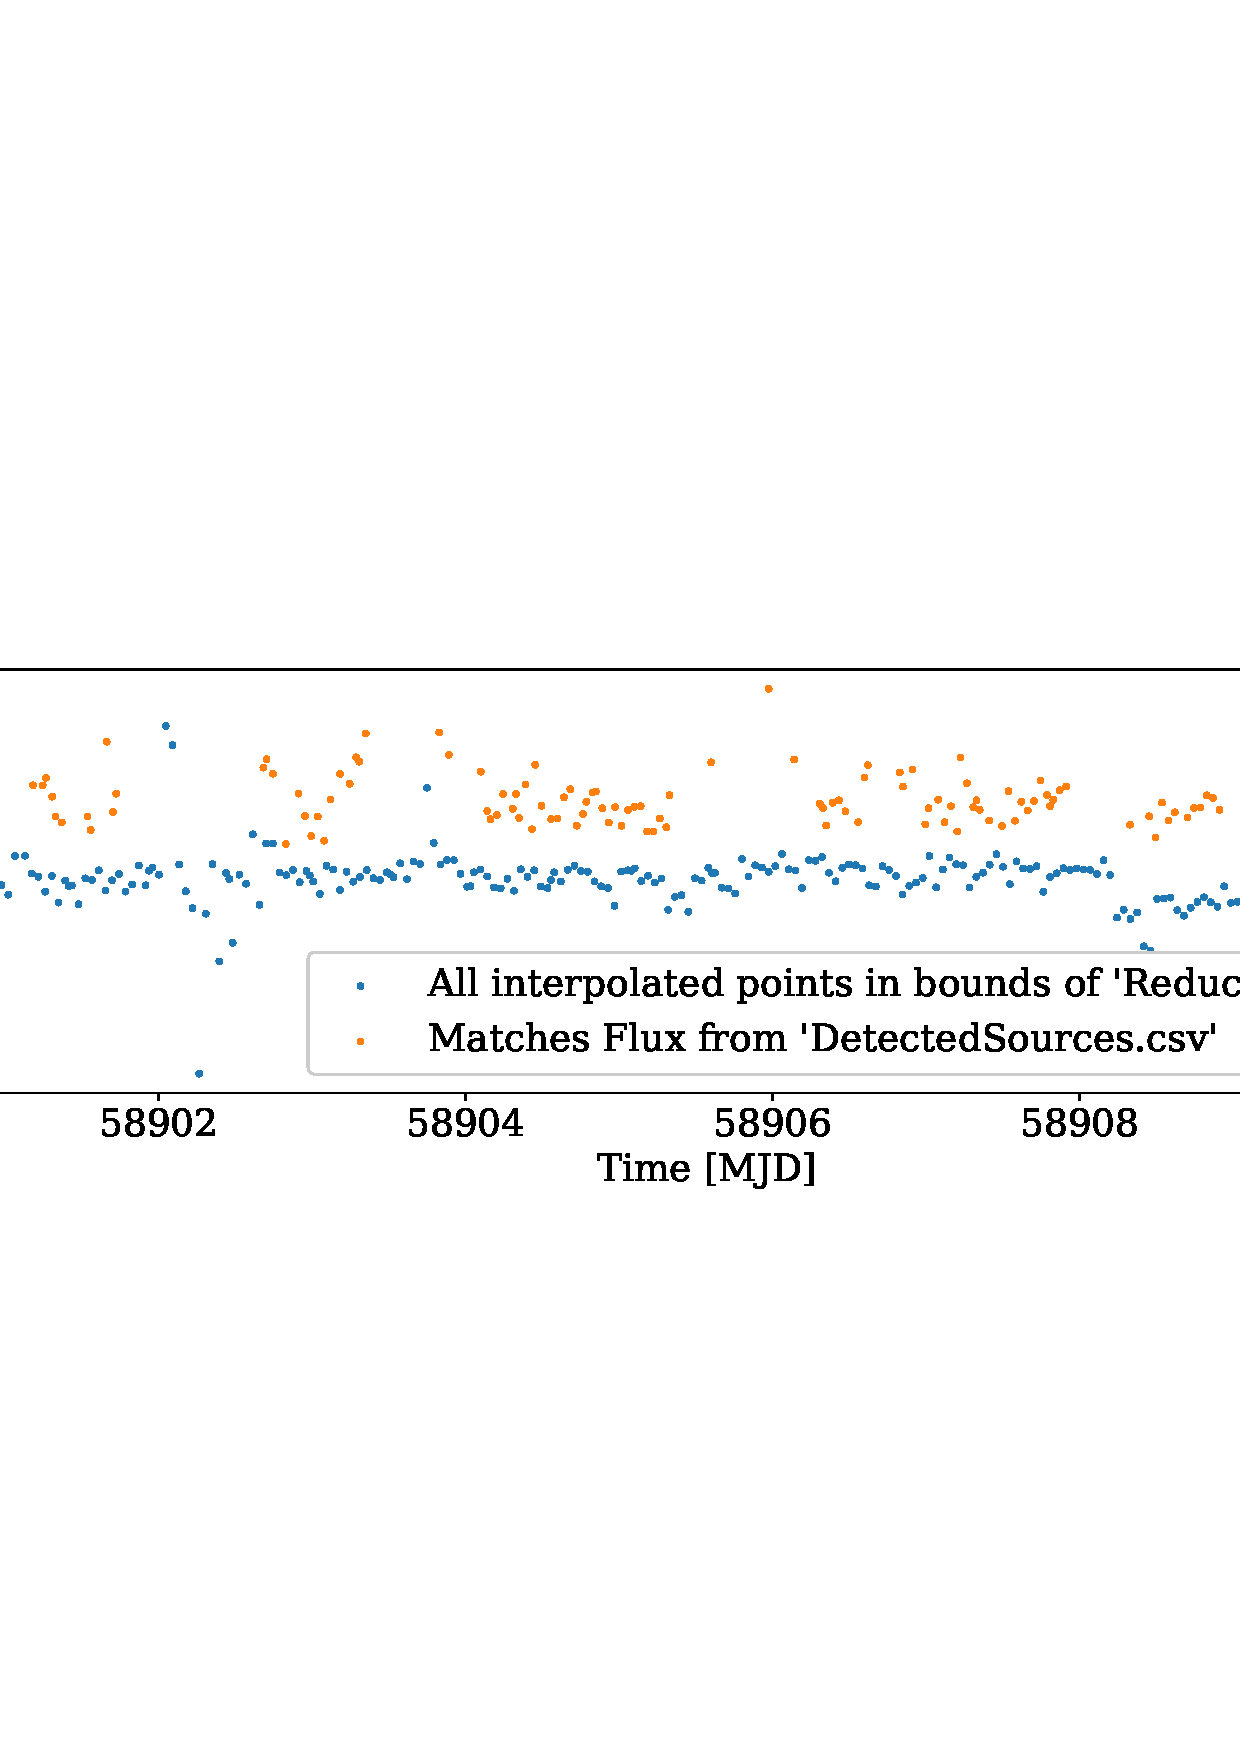
\includegraphics[width =\columnwidth]{../Test Code/Testing Figures/differentFluxes Ruff .pdf}
  \caption[Light curves of Ruff]{The light curves of the asteroid ``Ruff'', with the flux of the interpolated positions in blue circles and the flux from the matches to detected sources in orange diamonds.
  The Flux axis is measured in counts, as calculated by \texttt{TESSreduce}, and the times are in Modified Julian Date.}
  \label{Fig:DifFlux}
\end{figure}
    

\newpage %! Page number above here must be <=25

\section*{Acknowledgements}
%OzSTAR asks for:
\small
This work was performed on the OzSTAR national facility at Swinburne University of Technology. 
The OzSTAR program receives funding in part from the Astronomy National Collaborative Research Infrastructure Strategy (NCRIS) allocation provided by the Australian Government, and from the Victorian Higher Education State Investment Fund (VHESIF) provided by the Victorian Government.


%*Bib
\bibliographystyle{jphysicsB}
\bibliography{bibfile.bib}
\end{document}



